\section{Strengths and limitations}

Non-local means finds benefit in image with less texture
(that is, less diversity in colours).
Figure \ref{fig:ex-1} shows this clearly.
In the image, 
there is some highly textured hills that are minimally effected by
non-local means; however,
the sky that is more smooth is denoised effectively without losing too much detail.
We also see that median filtering is not as effective at removing noise in 
either scenario. and causes quite a lot of detail to be lost.

\begin{figure}
    \centering
    \includegraphics[width=0.7\linewidth]{images/ex-1-original.jpg}
    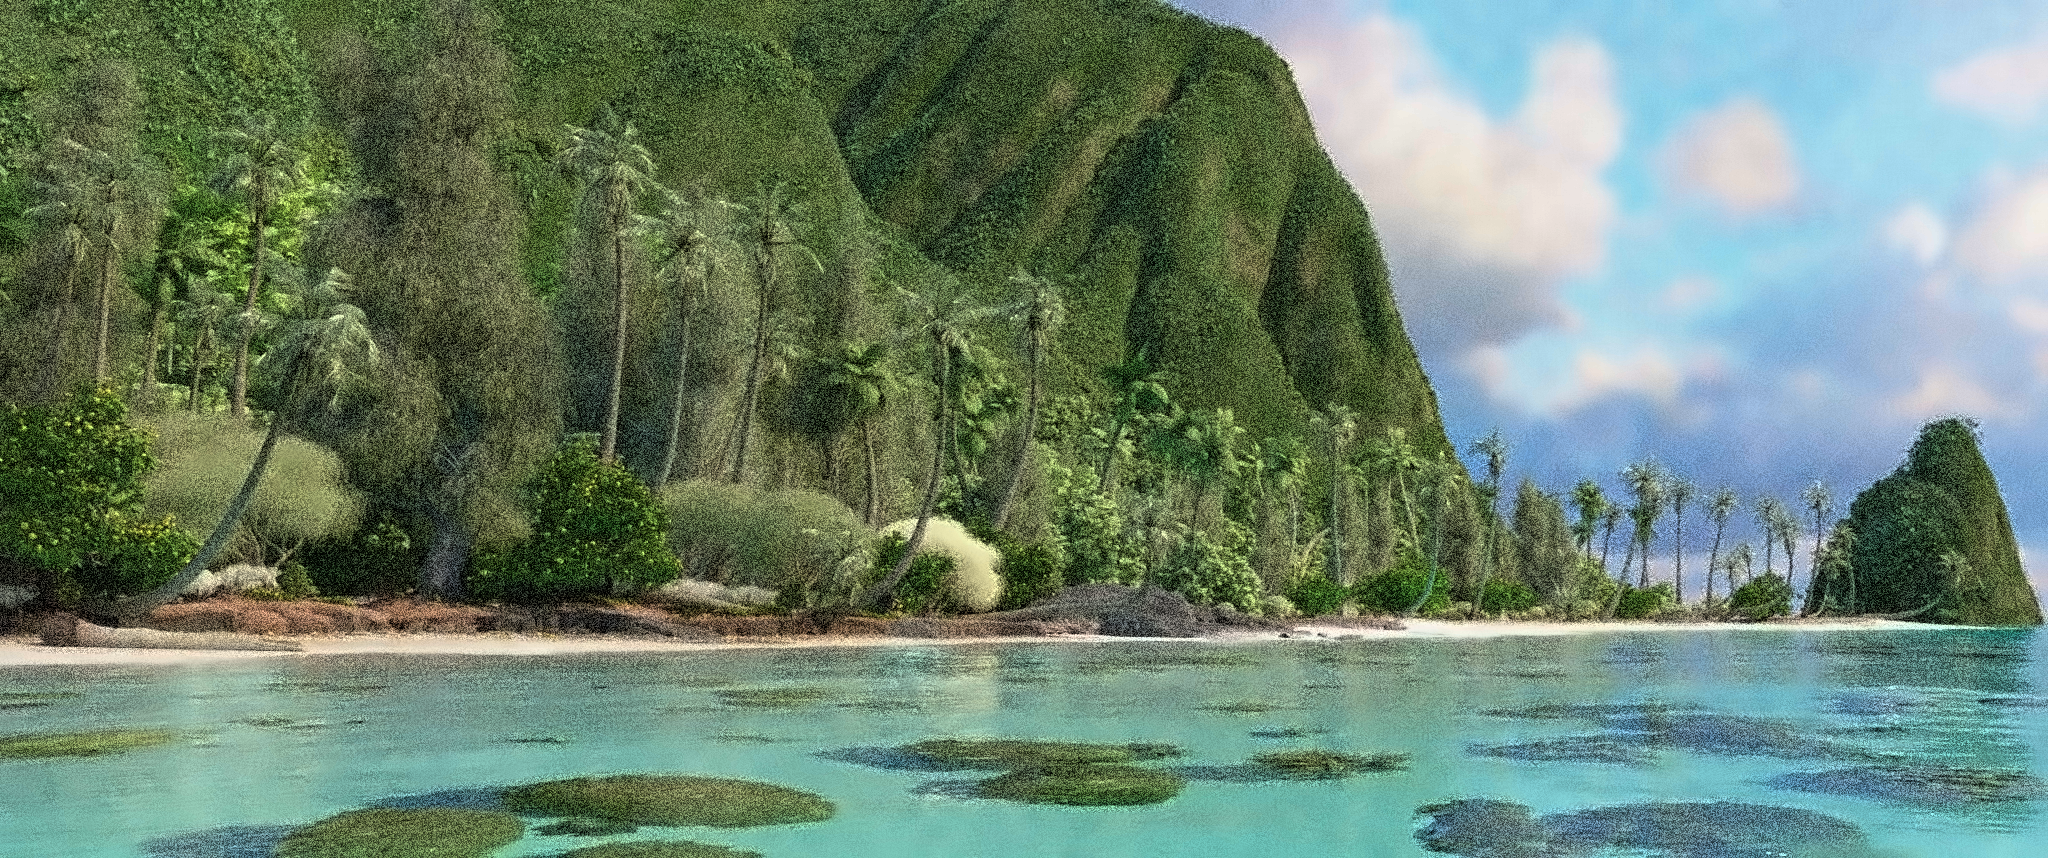
\includegraphics[width=0.7\linewidth]{images/ex-1-denoise.png}
    \includegraphics[width=0.7\linewidth]{images/ex-1-median.png}
    \caption{An example of non-local means on an image with uniform noise.
             The top image is the original, 
             then the image with non-local means, 
             and then the image with median filter.}
    \label{fig:ex-1}
\end{figure}

Non-local means adds a \emph{method noise} to images,
this looks like white which is \emph{typically} not as severe
as noise generated from other denoising methods \cite{buades2004image}.

\subsection{Salt and pepper noise}

Median filter and adaptive median filter are established techniques for
reducing salt and pepper noise for low variance; however, non-local means
has shown to be effective algorithm for denoising salt and pepper noise
even for high variance values. One note on this research is the high
computation time needed to apply the non-local means filter, this has been
noted as a point of future work \cite{sarker2012use}.

\subsection{Limiations}

\paragraph{Staircasing effect}

In non-local means and other neighbourhood filters 
(that is, the bilateral filter and the sigma filter)
there is a \emph{staircasing effect} that is observed.
This is the creation of flat regions in the image separated by artifact boundaries.
There exists a subjacent stade partial differential equations that can be solved to provide a solution
for this effect, presented by A. Buades et al. \cite{buades2006staircasing}.
